\documentclass[10pt, a4paper]{article} % use larger type; default would be 10pt

\usepackage{fontspec} % Font selection for XeLaTeX; see fontspec.pdf for documentation
\defaultfontfeatures{Mapping=tex-text} % to support TeX conventions like ``---''
\usepackage{xunicode} % Unicode support for LaTeX character names (accents, European chars, etc)
\usepackage{xltxtra} % Extra customizations for XeLaTeX
\usepackage{tikz}
% \usepackage{coloremoji}
\usetikzlibrary{arrows,calc,patterns}


% other LaTeX packages.....
\usepackage{fullpage}
\usepackage[top=2cm, bottom=4.5cm, left=2.5cm, right=2.5cm]{geometry}
\usepackage{amsmath,amsthm,amsfonts,amssymb,amscd,systeme}
\usepackage{unicode-math}
\usepackage{cancel}
\geometry{a4paper} 
%\usepackage[parfill]{parskip} % Activate to begin paragraphs with an empty line rather than an indent
\usepackage{fancyhdr}
\usepackage{listings}
\usepackage{graphicx}
\usepackage{hyperref}
\usepackage{multicol}

\usepackage{xcolor}

% FONTS
% \setmainfont[Ligatures=TeX]{Cambria Math} % set the main body font (\textrm), assumes Charis SIL is installed
%\setsansfont{Deja Vu Sans}
% \setmonofont[Ligatures=TeX]{Fira Code}
\setmathfont[Ligatures=TeX]{NewCMMath-Regular}

\setmainfont{Cambria}
\setmonofont[Ligatures=TeX]{Roboto Mono}

\renewcommand\lstlistingname{Algorithm}
\renewcommand\lstlistlistingname{Algorithms}
\def\lstlistingautorefname{Alg.}
\lstdefinestyle{mystyle}{
    % backgroundcolor=\color{backcolour},   
    % commentstyle=\color{codegreen},
    % keywordstyle=\color{magenta},
    % numberstyle=\tiny\color{codegray},
    % stringstyle=\color{codepurple},
    basicstyle=\ttfamily\footnotesize,
    breakatwhitespace=false,         
    breaklines=true,                 
    captionpos=b,                    
    keepspaces=true,                 
    numbers=left,                    
    numbersep=5pt,                  
    showspaces=false,                
    showstringspaces=false,
    showtabs=false,                  
    tabsize=2
}
\lstset{style=mystyle}

\newcommand\course{MS1 - Differential geometry and topology}
\newcommand\hwnumber{Контрольна Робота 1}                   % <-- homework number
\newcommand\idgroup{111-2023}                
\newcommand\idname{Михайло Корешков}  

\usepackage[framemethod=TikZ]{mdframed}
\mdfsetup{%
	backgroundcolor = black!5,
}
\mdfdefinestyle{ans}{%
    backgroundcolor = green!5,
    linecolor = green!50,
    linewidth = 1pt,
}

\pagestyle{fancyplain}
\headheight 35pt
\lhead{\idgroup \\ \idname}
\chead{\textbf{\Large \hwnumber}}
\rhead{\course \\ \today}
\lfoot{}
\cfoot{}
\rfoot{\small\thepage}
\headsep 1.5em

\linespread{1.2}

\newcommand{\R}{\mathbb{R}}
\newcommand{\N}{\mathbb{N}}
\newcommand{\Z}{\mathbb{Z}}
\newcommand{\J}{J}
\DeclareMathOperator{\lcm}{lcm}
\DeclareMathOperator{\cd}{CD}
\DeclareMathOperator{\id}{id}
\DeclareMathOperator{\rank}{rank}

\renewcommand{\B}{\mathcal{B}}

\newtheorem*{definition}{Визначення}

\newcommand{\todo}[1]{\colorbox{red}{\textbf{TODO}: #1}}


\begin{document}

\section*{Ex 1.1}
\begin{mdframed}
    Показати що відображення 
    \[\phi: B_1(0) \to \R^n; \quad \phi(x)=\frac{x}{1-|x|^2}\]
    є $C^\infty$ дифеоморфізмом.

    Дослідити двовимірний випадок.
    \[\phi(x,y) = \left(\frac{x}{1-x^2-y^2}, \frac{y}{1-x^2-y^2}\right), \quad (x,y)\in\R^2\]

    Знайти обернене відображення
\end{mdframed}

\subsection*{Ex 1.1.1. Обернене відображення}

Let 

\[f(x) = \frac{x}{1-|x|^2}, \quad \phi : B_{1}(0) \to \R^n\]
\[|x|^2 := r^2\]
\[|f(x)| = |y| := p = \frac{r}{1-r^2}\]
Можна отримати рівняння
\[pr^2+r-p=0\]
З цього виражаємо норму $x$ ($r$) через норму $f(x)$ ($p$).
\[r = \frac{\sqrt{1+4p^2}-1}{2p}\]
Далі використовуємо той факт, що вектори $x$ та $f(x)$ пропорційні
\[x = \frac{y}{|y|}\cdot r = y \cdot \frac{r}{p} = y \cdot \frac{\sqrt{1+4p^2}-1}{2p^2}\]

\begin{mdframed}[backgroundcolor=green!20]
    Отже, обернене відображення має вигляд
    \[f^{-1}(y) = y \cdot \frac{\sqrt{1+4|y|^2}-1}{2|y|^2}, \quad f^{-1} : \R^n \to B_1(0)\]
\end{mdframed}

\subsection*{Ex 1.1.2. $f$ - бієктивне}
\subsubsection*{Ін'єктивність}

Нехай
\[k(r) = \frac{1}{1-r^2}, \quad k: [0;1) \to \R\]
Припустимо, що $k(p)=k(q) \in \R$.
\[\frac{1}{1-p^2} = \frac{1}{1-q^2}, \quad (1-p^2) > 0, \quad (1-q^2) > 0\]
\[1-q^2 = 1-p^2\]
\[\begin{cases}
    q^2 = p^2 \\
    q,p \ge 0
\end{cases} \implies p=q\]
Тобто $k(r)$ - ін'єктивна.

З існування оберненого випливає сюр'єктивність.
Тобто $k(r) : [0;1) \to \R$ - бієкція.

Припустимо, що $f(x)=f(y)$.
% Знаємо, що $\forall x \in B_1(0): \; f(x) = k(x) \cdot x$ та $k(x) \ge 0$, тобто $f(x)$ пропорційний $x$ та направлений в один бік. 

\[\frac{x}{1-|x|^2} = \frac{y}{1-|y|^2}\]
\[x = y \cdot \frac{1-|x|^2}{1-|y|^2}\]
Тобто $x$ та $y$ пропорційні з коефіцієнтом $\frac{1-|x|^2}{1-|y|^2} > 0$.

\[\frac{|x|}{1-|x|^2} = \frac{|y|}{1-|y|^2}\]
\[|x|-|x||y|^2 = |y|-|x|^2|y|\]
\[|x|-|y|+|x||y|(|x|-|y|) = (|x|-|y|)(1+|x||y|) = 0\]
\[1 + |x||y| > 0\]
Отже
\[|x|=|y|\]

Оскільки $x$ та $y$ пропорційні та направлені в один бік, то це еквівалентно $x=y$.
Тобто довели ін'єктивність у вигляді $f(x)=f(y) \implies x=y$

Сюр'єктивність $f$ випливає з існування оберненого.

\subsection*{Ex 1.1.2. $C^k$-дифеоморфізм}
\todo{Доведення не закінчено!!!}\\
\todo{привести в порядок доведення. порахувати матрицю якобі та спробувати порахувати її визначник.}
Покладемо
\[\phi(x) = x \cdot k(|x|)\]
\[k(r) = \frac{1}{1-r^2}, \quad k : [0,1) \to \R\] 
\[l(r) = 1-r^2, \quad l : [0,1) \to (0,1], \quad l\in C^k\]
\[k(r) = \frac{1}{l(r)}\]

% \[k'(x) = -\frac{-2x}{(1-|x|^2)^2} = 2x(1-|x|^2)^{-2} = 2x \cdot k^2(x)\]
% \[k'(x) = 2x\cdot k^2(x)\]

% \[k^{(2)}(x) = 2(1-|x|^2)^{-2} + 8x^2(1-|x|^2)^{-3} = 2k^2(x) + 8x^2\cdot k^3(x)\]
% \[k^{(n+1)}(x) = (k')^{(n)} = \sum_{k=0}^n C_n^k (2x)^{(k)}\cdot k^{(n-k)}\]

Хочу довести монотонність $k(r)$. Нехай $0\le a<b < 1$.
\[a<b \implies a^2 < b^2 \implies 1-a^2 > 1-b^2\]
\[\frac{k(b)}{k(a)} = \frac{1-a^2}{1-b^2} > \frac{1-b^2}{1-b^2} = 1 \]
Тобто $k(r)$ - монотонно зростаюча.

В попередньому пункті фактично довели, що вона сюр'єктивна.

Зауважу, що $l(r)=1-r^2 \in C^\infty$ і $\forall r \in [0,1): l(r) \ne 0$.
З цього, $k(r) = 1/l(r) \in C^\infty$

\[k'(r) = \frac{2r}{(1-r^2)^2}\]
\[\forall r>0: k'(r) > 0\]
\[k'(0) = 0\]

\begin{mdframed}[backgroundcolor=purple!20]
    \textbf{Лема Адамара} (трошки модифікована під наш випадок)

    Нехай 
    \[k : B^n_1(0) \to \R, \quad B^n_1(0) \subset \R^n, \quad k \in C^\infty\]
    
    Тоді існують $n$ відображень $g_i$ таких що 
    \begin{align*}
        & g_i : B^n_1(0) \to \R, \quad g_i \in C^\infty;\\
        & g(x) := (g_1(x), ..., g_n(x))\\
        & f(x) = f(\vec 0) + (x, g(x)) 
    \end{align*}
    Де $(x,g(x)) = \sum_i x_ig_i(x)$.
\end{mdframed}

Тоді 
\[\frac{1}{1-|x|^2} = \frac{1}{1-|\vec 0|^2} + (x, g(x)) = 1 + (x, g(x)), \quad g_i(x)\in C^\infty\]

Повертаємось до $\phi(x)$:
\[\phi(x) = x \cdot \frac{1}{1-|x|^2} = x \cdot (1 + (x, g(x))) = x + x(x,g(x))\]

Тут і далі використовується нотація підсумовування за Ейнштейном ($a_ib_i := \sum_i a_ib_i$).
\begin{align*}
    J_{ij} &= \partial_j (x_i(1+(x,g(x)))) = \partial_j (x_i(1+x_kg_k(x))) = \\
    & = \delta^j_i (1+x_kg_k(x)) + x_i \partial_j (x_kg_k(x))
\end{align*}

Підставляємо $x=\vec 0$ і отримуємо
\begin{align*}
    J_{ij}(\vec 0) &= \delta^j_i (1+\cancelto{0}{x_k}g_k(x)) + \cancelto{0}{x_i} \cdot \partial_j (x_kg_k(x)) = \\
    & = \delta_{ij}
\end{align*}

Тобто маємо повний ранг оператора $\phi$ в нулі.

\subsubsection*{Підсумовуємо}

\begin{itemize}
    \item $k(r) = \frac{1}{1-r^2} : [0,1) \to [0,+\infty)$ - строго монотонне бієктивне $C^k$-відображення
    \item $\phi(x) = x \cdot k(|x|)$ - бієктивне $C^k$ відображення, гомеоморфізм
    \item $\phi$ має повний ранг в точці $\vec 0$ за вищевказаним доведенням
    \item $\phi$ має повний ранг в інших точках, бо $k'(|x|) > 0$ (трошки махання руками)
\end{itemize}

Отже, $\phi$ має бути $C^\infty$-дифеоморфізмом 



\section*{Ex 1.2}
\subsection*{Ex 1.2.1}
\begin{mdframed}
    Нехай $\alpha = \{(U_i,\phi_i)\}$ - $C^k$ атлас на $X$.\\
    Нехай $\beta = \{(V_i,\psi_i)\}$ - сім'я попарно $C^k$-узгоджених локальних карт.\\
    Довести що наступне еквівалентно 
    \begin{itemize}
        \item $\alpha$ та $\beta$ є $C^k$-узгодженими
        \item $\alpha\cup\beta$ є $C^k$ атласом на $X$
    \end{itemize}
\end{mdframed}

\begin{definition}[$C^k$-атлас]
    $\alpha = \{(U_{i}, \phi_{i}\})_{i\in I}$ - це  $C^k$-Атлас многовиду якщо
    \[\forall (U,\phi), (V,\psi) \in \alpha: (U\cap V \ne \varnothing) \implies \left(\phi\circ\psi^{-1}, \psi\circ\phi^{-1} \in C^k\right)\]
    Де 
    \begin{gather*}
        \phi\circ\psi^{-1} : \psi(U\cap V) \to \phi(U\cap V)\\
        \psi\circ\phi^{-1} : \phi(U\cap V) \to \psi(U\cap V)\\
    \end{gather*}
\end{definition}

\begin{proof}[Доведення 1->2]
    $\alpha$ та $\beta$ є $C^k$-узгодженими.
    Тоді 
    \[\forall (U,\phi) \in \alpha, (V,\psi) \in \beta: \phi \circ \psi^{-1}, \psi \circ \phi^{-1} \in C^k\]
    Але з визначення узгодженого атласу та умови, що всі локальні карти $\beta$ попарно узгоджені: 
    \[\forall (U,\phi),(V,\psi) \in (\alpha\cup\beta): \]
    \[\left[\begin{array}{ll}
        (U,\phi),(V,\psi) \in \alpha &\implies \phi\circ\psi^{-1}, \psi \circ \phi^{-1} \in C^k,\quad \text{as $\alpha$ is a $C^k$-atlas} \\
        (U,\phi),(V,\psi) \in \beta &\implies \phi\circ\psi^{-1}, \psi \circ \phi^{-1} \in C^k,\quad \text{from definition of } \beta \\
        (U,\phi) \in \alpha, (V,\psi) \in \beta & \implies \phi\circ\psi^{-1}, \psi \circ \phi^{-1} \in C^k, \quad \text{because $\alpha$ and $\beta$ are $C^k$-related} 
    \end{array}\right.\]

    Таким чином, $\alpha\cup\beta$ - дійсно $C^k$ атлас.
\end{proof}

\begin{proof}[Доведення 2->1]
    $\alpha\cup\beta$ є $C^k$-атласом.
    Тоді 
    \[\forall (U,\phi),(V,\psi) \in (\alpha\cup\beta): \phi \circ \psi^{-1}, \psi \circ \phi^{-1} \in C^k\]
    А тоді 
    \[\forall (U,\phi) \in \alpha\subset (\alpha\cup\beta), (V,\psi) \in \beta \subset (\alpha\cup\beta): \phi \circ \psi^{-1}, \psi \circ \phi^{-1} \in C^k\]
    Таким чином, $\alpha$ та $\beta$ - дійсно $C^k$ узгоджені.
\end{proof}

\subsection*{Ex 1.2.2}
\begin{mdframed}
    Довести, що $C^k$ узгодженість це відошення еквівалентності на множині $C^k$ атласів
\end{mdframed}
Розглядаємо атласи многовиду $M$.
\begin{proof}
    \begin{itemize}
        \item \textbf{Рефлексивність}\\
        $\alpha$ узгоджений з $\alpha$ бо $\alpha\cup\alpha=\alpha$ є $C^k$ атласом (за задачею 1.2.1)
        \item \textbf{Симетричність} - очевидна
        \item \textbf{Транзитивність}\\
        $\alpha,\beta$ - узгоджені, $\beta,\gamma$ - узгоджені.
        Нехай $(U,x)\in\alpha, \; (W,z)\in\gamma, \; U\cap W \ne \varnothing$. \\
        
        % Нехай точка $p \in U\cap W \subset M$. \\
        % Тоді для точки $p$ беремо деяку локальну карту $(V, y) \in \beta$.
        % Множина $U\cap V \cap W$ буде також відкритим околом $p$.

        Для будь якої $p \in U\cap W: \exists (y_p, V_p) \in \beta, \; p\in V_p$.
        Тоді $\forall p \in U\cap W:$
        \begin{gather*}
            x : U \to x(U), \quad y : V_p \to y(V_p), \quad z : W \to z(W).\\
            x \circ y_p^{-1} : y(U\cap V_p) \to x(U\cap V_p) \in C^k\\
            y_p \circ z^{-1} : z(V_p\cap W) \to y(V_p\cap W) \in C^k
        \end{gather*}

        Далі розглянемо обмеження відображень на $U\cap V_p \cap W$
        \begin{gather*}
            U\cap V_p\cap W \subset U\cap V_p, V_p\cap W\\
            x \circ y_p^{-1} : y_p(U\cap V_p\cap W) \to x(U\cap V_p\cap W) \in C^k\\
            y_p \circ z^{-1} : z(U\cap V_p\cap W) \to y_p(U\cap V_p\cap W) \in C^k\\
            \implies\\
            \forall p\in U\cap W:\; x \circ y_p^{-1} \circ y_p \circ z^{-1} = x \circ z^{-1} : z(U\cap V_p\cap W) \to x(U\cap V_p\cap W) \in C^k
        \end{gather*}

        Позначимо 
        \[A_p := U\cap V_p\cap W\]
        \[\phi_p := \left(x \circ z^{-1}\right)|_{A_p}, \quad \phi_p : z(A_p) \to x(A_p) \]
        
        Таким чином для будь якої точки перетину $p\in U\cap W$ існує свій $C^\infty$ відображення переходу $\phi_p$.
        Залишається довести, що всі $\phi_p$ узгоджені між собою, тобто
        \[\left(x \circ z^{-1}\right)(z(p)) = \phi_p(z(p)) \in C^{\infty}\]

        % Маємо
        % \[U\cap W = \bigcup_p A_p\]
        % Далі
        % \[\forall p,t \in U \cap W: \exists \begin{cases}
        %     \phi_p : z(A_p) \to x(A_p)\\
        %     \phi_t : z(A_t) \to x(A_t)
        % \end{cases}\]

        \todo{Питання в тому, як показати, що відображення $\left(x \circ z^{-1}\right)(z(p)) = \phi_p(z(p))$} 
        \todo{дійсно $C^k$ дифеоморфізм в усій області $U\cap W$. }
        \todo{Чи вистачає того, що воно є таким за побудовою в кожному околі точки $p$?}

        % Питання в тому як подовжити відображення $x \circ z^{-1}$ на $z(U\cap W) \to x(U\cap W)$.
    \end{itemize}
\end{proof}

\subsection*{Ex 1.2.3}
\begin{mdframed}
    Показати що об'єднання попарно $C^k$-узгоджених $C^k$-атласів 
    \[\alpha = \bigcup_{i\in I} \alpha_i\] 
    є $C^k$-атласом, $C^k$-узгодженим з кожним $\alpha_i$.
\end{mdframed}

\begin{proof}
    
Спершу доведу, що $\alpha$ - дійсно $C^k$-атлас.

$\forall i,j\in I: \alpha_i \cup \alpha_j$ - це $C^k$-атлас (з пункту 1). З цього маємо, що всі скінченні об'єднання $\alpha_i$ будуть $C^k$-атласами.

Візьмемо довільні локальні карти $(U,x), (V,y) \in \alpha$.\\
$\exists i,j\in I: (U,x) \in \alpha_i, \; (V,y)\in\alpha_j$\\
Маємо, що карти $(U,x)$ та $(V,y)$ $C^k$-узгоджені, бо $C^k$-узгодженими є атласи $\alpha_i$ та $\alpha_j$ (в тому числі коли $i=j$).\\
Тобто, $\alpha$ - дійсно $C^k$-атлас.

З пункту 1 маємо, що $\forall k: \alpha \cup \alpha_k = \alpha$ - $C^k$-атлас, а отже $\forall k: \alpha_k$ є $C^k$-узгодженим з $\alpha$.

\end{proof}

\section*{Ex 1.3}
\begin{mdframed}
    Показати, що 
    \[f : \R^m \to \R^n\]
    є диференційовним класу $k$ в звичайному сенсі тітт коли 
    \[f_1: (\R^m, \id_m) \to (\R^n, \id_n) \in C^k\]
    у сенсі відображення між многовидами зі канонічною гладкою структурою
\end{mdframed}

\begin{proof}[Доведення]
    Нехай $f \in C^k$.
    Розглянемо визначення $C^k$ відображення у сенсі многовидів. $f_1 \in C^k$ якщо
    \[\id_n \circ f \circ \id_m^{-1} : \R^m \to \R^n \in C^k \]
    Де ліворуч та праворуч композиція з картами відповідних многовидів, які в канонічному варіанті є просто тотожними відображеннями.
    Маємо
    \[\id_n \circ f \circ \id_m^{-1} = f \in C^k\]
    Тобто виконано умову $C^k$ гладкості відображення $f$ як відображення між многовидами.

    Звісно, тут також використано, що $\id_n$ та $\id_m$ є $C^\infty$-дифеоморфізмами та $\id = \id^{-1}$

    У зворотній бік аналогічно, але починаємо з $f : \R^m \to \R^n$ і додаємо композицію з $\id$ з боків.
\end{proof}

\section*{Ex 1.4}
\subsection*{Ex 1.4.1}
\begin{mdframed}
    \[f(x) = x^2\]
\end{mdframed}

\subsubsection*{a) Дотичне відображення}
\[Tf : T\R \to T\R\]
\begin{gather*}
    f'(x) = 2x\\
    \colorbox{yellow}{$Tf(x,v) = (f(x), f'(x)\cdot v) = (x^2, 2xv)$}
\end{gather*}

\subsubsection*{b) Критичні точки. Точки локального дифеоморфізму.}
Для цього знайдемо ранг матриці Якобі.
Матриця Якобі $\R\to\R$ є одним числом. $\rank Jf = [x=0]$.

Критичними точками будуть ті, де матриця Якобі матиме не повний ранг.\\
Тобто \colorbox{yellow}{єдина критична точка - $x=0$}.

Точки локального дифеоморфізму будуть тими, де матриця Якобі має повний ранг.
Тобто всюди окрім $x=0$ відображення $f$ буде локальним дифеоморфізмом.

\subsubsection*{c) Дотичне відображення - нульове}
\[T_{x}f : T_{x}\R \to T_{f(x)}\R\]
\begin{gather*}
    T_{x}f(v) = f'(x) \cdot v = 2xv\\
    \left(\forall v\in T_{x}\R: 2xv = 0\right) \implies  x = 0
\end{gather*}

Тобто \colorbox{yellow}{$T_{x}f \equiv 0$ лише для $x=0$}

\subsubsection*{d) Дотичне відображення - ізоморфізм}

\[\forall x\ne 0: T_{x}f(v) = (2x)\cdot v\]
Для $x\ne 0$ лінійне відображення $T_{x}f(v)$ діє між просторами однієї розмірності та має тривіальне ядро $\ker T_{x}f(v) = \{0\}$. \\
Тобто \colorbox{yellow}{$T_{x}f(v)$ - ізоморфізм для $x\ne 0$}

\todo{довести чому саме $f$ не буде ізоморфізмом для $x = 0$}

\subsection*{Ex 1.4.2}
\begin{mdframed}
    \[f(x) = \cos x\]
\end{mdframed}

\subsubsection*{a) Дотичне відображення}
\[Tf : T\R \to T\R\]
\begin{gather*}
    f'(x) = -\sin x\\
    \colorbox{yellow}{$Tf(x,v) = (f(x), f'(x)\cdot v) = (\cos x, -\sin x \cdot v)$}
\end{gather*}

\subsubsection*{b) Критичні точки. Точки локального дифеоморфізму.}
$\rank Jf = [-\sin x = 0] = [x = \pi k, k\in\mathbb Z]$.

Критичними точками будуть ті, де матриця Якобі матиме не повний ранг.\\
Тобто \colorbox{yellow}{критичні точки - $x \in \{\pi k : k\in\mathbb Z\}$}.

Точки локального дифеоморфізму будуть тими, де матриця Якобі має повний ранг.
Тобто всюди окрім таких де $\sin x = 0$ відображення $f$ буде локальним дифеоморфізмом.

\subsubsection*{c) Дотичне відображення - нульове}
\[T_{x}f : T_{x}\R \to T_{f(x)}\R\]
\begin{gather*}
    T_{x}f(v) = f'(x) \cdot v = -\sin x \cdot v\\
    \left(\forall v\in T_{x}\R: -\sin x \cdot v = 0\right) \implies  x \in \{\pi k : k\in\mathbb Z\}
\end{gather*}

Тобто \colorbox{yellow}{$T_{x}f \equiv 0$ для $x \in \{\pi k : k\in\mathbb Z\}$}

\subsubsection*{d) Дотичне відображення - ізоморфізм}

Для $x \notin \{\pi k : k\in\mathbb Z\}$ лінійне відображення $T_{x}f(v) = (-\sin x) \cdot v$ діє між просторами однієї розмірності та має тривіальне ядро $\ker T_{x}f(v) = \{0\}$. \\
Тобто \colorbox{yellow}{$T_{x}f(v)$ - ізоморфізм для $x \notin \{\pi k : k\in\mathbb Z\}$}

\todo{довести чому саме $f$ не буде ізоморфізмом для $x \in \{\pi k : k\in\mathbb Z\}$}

\subsection*{Ex 1.4.3}
\begin{mdframed}
    \[f(x) = x^3 - 1\]
\end{mdframed}

\subsubsection*{a) Дотичне відображення}
\[Tf : T\R \to T\R\]
\begin{gather*}
    f'(x) = 3x^2\\
    \colorbox{yellow}{$Tf(x,v) = (f(x), f'(x)\cdot v) = (x^3-1, 3x^2 \cdot v)$}
\end{gather*}

\subsubsection*{b) Критичні точки. Точки локального дифеоморфізму.}
$\rank Jf = [3x^2 = 0] = [x = 0]$.

Критичними точками будуть ті, де матриця Якобі матиме не повний ранг.\\
Тобто \colorbox{yellow}{одна критична точка - $x = 0$}.

Точки локального дифеоморфізму будуть тими, де матриця Якобі має повний ранг.
Тобто всюди окрім таких де $x = 0$ відображення $f$ буде локальним дифеоморфізмом.

\subsubsection*{c) Дотичне відображення - нульове}
\[T_{x}f : T_{x}\R \to T_{f(x)}\R\]
\begin{gather*}
    T_{x}f(v) = f'(x) \cdot v = 3x^2 \cdot v\\
    \left(\forall v\in T_{x}\R: 3x^2 \cdot v = 0\right) \implies  x=0
\end{gather*}

Тобто \colorbox{yellow}{$T_{x}f \equiv 0$ для $x=0$}

\subsubsection*{d) Дотичне відображення - ізоморфізм}

Для $x \ne 0$ лінійне відображення $T_{x}f(v) = (3x^2) \cdot v$ діє між просторами однієї розмірності та має тривіальне ядро $\ker T_{x}f(v) = \{0\}$. \\
Тобто \colorbox{yellow}{$T_{x}f(v)$ - ізоморфізм для $x\ne 0$}

\todo{довести чому саме $f$ не буде ізоморфізмом для $x = 0$}


\subsection*{Ex 1.4.4}
\begin{mdframed}
    \[f(x) = e^x\]
\end{mdframed}

\subsubsection*{a) Дотичне відображення}
\[Tf : T\R \to T\R\]
\begin{gather*}
    f'(x) = e^x\\
    \colorbox{yellow}{$Tf(x,v) = (f(x), f'(x)\cdot v) = (e^x, e^x \cdot v)$}
\end{gather*}

\subsubsection*{b) Критичні точки. Точки локального дифеоморфізму.}
$\rank Jf = [e^x = 0] = 1$ оскільки $\forall x\in\R: e^x > 0$.

Критичними точками будуть ті, де матриця Якобі матиме не повний ранг.\\
Тобто \colorbox{yellow}{критичних точок немає}.

Точки локального дифеоморфізму будуть тими, де матриця Якобі має повний ранг.\\
Тобто відображення $f$ буде локальним дифеоморфізмом всюди.

\subsubsection*{c) Дотичне відображення - нульове}
\[T_{x}f : T_{x}\R \to T_{f(x)}\R\]
\begin{gather*}
    T_{x}f(v) = f'(x) \cdot v = e^x \cdot v\\
    \forall v\in T_{x}\R: e^x \cdot v = 0
\end{gather*}
Такого не буває

Тобто \colorbox{yellow}{$\forall x\in\R: T_{x}f \nequiv 0$}

\subsubsection*{d) Дотичне відображення - ізоморфізм}

Лінійне відображення $T_{x}f(v) = e^x \cdot v$ діє між просторами однієї розмірності та має тривіальне ядро $\ker T_{x}f(v) = \{0\}$. \\
Тобто \colorbox{yellow}{$T_{x}f(v)$ - ізоморфізм для $\forall x\in \R$}


\section*{Ex 1.5}
\subsection*{Ex 1.5.1}
\begin{mdframed}
    \[f(x,y) = x^2 + y^2\]
\end{mdframed}

\subsubsection*{a) Матриця Якобі}
\[\J f = \begin{pmatrix}
    f'_x(x,y) & f'_y(x,y)
\end{pmatrix} = \begin{pmatrix}
    2x & 2y
\end{pmatrix}\]

\subsubsection*{b) Формула дотичного відображення}
\[Tf : T\R^2 \to T\R\]
\[(Tf)\left(\begin{pmatrix} x \\ y \end{pmatrix}, \begin{pmatrix} u \\ v \end{pmatrix}\right) 
= \left(f(x,y),\J f \begin{pmatrix} u \\ v \end{pmatrix}\right) 
= \left(x^2+y^2, 2xu+2yv\right)\]

\subsubsection*{c) Ранг дотичного відображення в точці}
\[T_{x,y} f : T_{x,y}\R^2 \to T_{f(x,y)}\R\]
\[(T_{x,y} f) \begin{pmatrix} u \\ v \end{pmatrix}
= J\begin{pmatrix} u \\ v \end{pmatrix} = f'_x(x,y) u + f'_y(x,y) v = 2xu+2yv\]

Відображення $J$ має ранг 0 коли обертається в константний 0, тобто коли обидва коефіцієнти нульові.
Іншими словами
\[\rank J = 0 \iff f'_x(x,y)=f'_y(x,y)=0\]
Тоді для рангу 1 справедливо
\[\rank J = 1 \iff f'_x(x,y)f'_y(x,y) \ne 0\]
Ранг більше 1 бути не може.

Точки рангу 0
\[2x=2y=0\]
\colorbox{yellow}{$(0,0)$ - єдина точка рангу 0}

Точки рангу 1
\[(x,y) \in \R^2 \setminus \{(0,0)\}\]

\subsubsection*{d) Критичні точки відображення $f$}

Точка є критичною коли ранг матриці Якобі менше максимально можливого, тобто менше 1. 
Таким чином критичними точками будуть точки рангу 0 з попереднього пункту

\subsubsection*{e) Точки, в яких $f$ є локальним дифеоморфізмом}
\todo{todo довести чому саме в критичних точках не буде дифеоморфізму}


\subsection*{Ex 1.5.2}
\begin{mdframed}
    \[f(x,y) = xy\]
\end{mdframed}

\subsubsection*{a) Матриця Якобі}
\[\J f = \begin{pmatrix}
    f'_x(x,y) & f'_y(x,y)
\end{pmatrix} = \begin{pmatrix}
    y & x
\end{pmatrix}\]

\subsubsection*{b) Формула дотичного відображення}
\[Tf : T\R^2 \to T\R\]
\[(Tf)\left(\begin{pmatrix} x \\ y \end{pmatrix}, \begin{pmatrix} u \\ v \end{pmatrix}\right) 
= \left(f(x,y),\J f \begin{pmatrix} u \\ v \end{pmatrix}\right) 
= \left(xy, yu+xv\right)\]

\subsubsection*{c) Ранг дотичного відображення в точці}
\[T_{x,y} f : T_{x,y}\R^2 \to T_{f(x,y)}\R\]
\[(T_{x,y} f) \begin{pmatrix} u \\ v \end{pmatrix}
= J\begin{pmatrix} u \\ v \end{pmatrix} = f'_x(x,y) u + f'_y(x,y) v = yu+xv\]

Точки рангу 0
\[x=y=0\]
\colorbox{yellow}{$(0,0)$ - єдина точка рангу 0}

Точки рангу 1
\[(x,y) \in \R^2 \setminus \{(0,0)\}\]

\subsubsection*{d) Критичні точки відображення $f$}

Критичними точками будуть точки рангу 0 з попереднього пункту

\subsubsection*{e) Точки, в яких $f$ є локальним дифеоморфізмом}
\todo{todo довести чому саме в критичних точках не буде дифеоморфізму}


\subsection*{Ex 1.5.3}
\begin{mdframed}
    \[f(x,y) = x^3 - xy\]
\end{mdframed}

\subsubsection*{a) Матриця Якобі}
\[\J f = \begin{pmatrix}
    f'_x(x,y) & f'_y(x,y)
\end{pmatrix} = \begin{pmatrix}
    2x^2-y & -x
\end{pmatrix}\]

\subsubsection*{b) Формула дотичного відображення}
\[Tf : T\R^2 \to T\R\]
\[(Tf)\left(\begin{pmatrix} x \\ y \end{pmatrix}, \begin{pmatrix} u \\ v \end{pmatrix}\right) 
= \left(f(x,y),\J f \begin{pmatrix} u \\ v \end{pmatrix}\right) 
= \left(x^3 - xy, (2x^2-y)u - xv\right)\]

\subsubsection*{c) Ранг дотичного відображення в точці}
\[T_{x,y} f : T_{x,y}\R^2 \to T_{f(x,y)}\R\]
\[(T_{x,y} f) \begin{pmatrix} u \\ v \end{pmatrix}
= J\begin{pmatrix} u \\ v \end{pmatrix} = f'_x(x,y) u + f'_y(x,y) v = (2x^2-y)u - xv\]

Точки рангу 0
\[(2x^2-y)=x=0\]
\[\begin{cases}
    x = 0\\
    y = 2x^2 = 0
\end{cases}\]
\colorbox{yellow}{$(0,0)$ - єдина точка рангу 0}

Точки рангу 1
\[(x,y) \in \R^2 \setminus \{(0,0)\}\]

\subsubsection*{d) Критичні точки відображення $f$}

Критичними точками будуть точки рангу 0 з попереднього пункту

\subsubsection*{e) Точки, в яких $f$ є локальним дифеоморфізмом}
\todo{todo довести чому саме в критичних точках не буде дифеоморфізму}


\subsection*{Ex 1.5.4}
\begin{mdframed}
    \[f(x,y) = \sin(x^2+y^2)\]
\end{mdframed}

\subsubsection*{a) Матриця Якобі}
\[\J f = \begin{pmatrix}
    f'_x(x,y) & f'_y(x,y)
\end{pmatrix} = \begin{pmatrix}
    2x\cos(x^2+y^2) & 2y\cos(x^2+y^2)
\end{pmatrix}\]

\subsubsection*{b) Формула дотичного відображення}
\[Tf : T\R^2 \to T\R\]
\[(Tf)\left(\begin{pmatrix} x \\ y \end{pmatrix}, \begin{pmatrix} u \\ v \end{pmatrix}\right) 
= \left(f(x,y),\J f \begin{pmatrix} u \\ v \end{pmatrix}\right) 
= \left(\sin(x^2+y^2), 2x\cos(x^2+y^2)u + 2y\cos(x^2+y^2)v\right)\]

\subsubsection*{c) Ранг дотичного відображення в точці}
\[T_{x,y} f : T_{x,y}\R^2 \to T_{f(x,y)}\R\]
\[(T_{x,y} f) \begin{pmatrix} u \\ v \end{pmatrix}
= J\begin{pmatrix} u \\ v \end{pmatrix} = f'_x(x,y) u + f'_y(x,y) v = 2x\cos(x^2+y^2)u + 2y\cos(x^2+y^2)v\]

Точки рангу 0
\[2x\cos(x^2+y^2)=2y\cos(x^2+y^2)=0\]
\[\left[\begin{array}{l}
    x=y=0\\
    \cos(x^2+y^2) = 0
\end{array}\right. \implies \left[\begin{array}{l}
    x=y=0\\
    x^2+y^2 = \frac{\pi}{2}+\pi k, k \in \mathbb Z
\end{array}\right. \]
\colorbox{yellow}{Ранг 0 мають точки $\{(0,0)\} \cup \{(x,y) : x^2+y^2 = \frac{\pi}{2}+\pi k, k \in \mathbb Z\}$}

Точки рангу 1 - всі інші

\subsubsection*{d) Критичні точки відображення $f$}

Критичними точками будуть точки рангу 0 з попереднього пункту

\subsubsection*{e) Точки, в яких $f$ є локальним дифеоморфізмом}
\todo{todo довести чому саме в критичних точках не буде дифеоморфізму}

\section*{Ex 1.6}

\subsection*{Ex 1.6.1}
\[f(x,y) = (x,y^2)\]
\subsubsection*{a) Матриця Якобі}
\begin{align*}
    Jf = \begin{pmatrix}
        (f|_x)'_x & (f|_x)'_y\\
        (f|_y)'_x & (f|_y)'_y
    \end{pmatrix} 
    = \begin{pmatrix}
        1 & 0\\
        0 & 2y
    \end{pmatrix}
\end{align*}

\subsubsection*{b) Формула дотичного відображення}
\[Tf : T\R^2 \to T\R^2\]
\[J\begin{pmatrix}u\\v\end{pmatrix} = \begin{pmatrix}u\\2yv\end{pmatrix}\]
\begin{align*}
    (Tf)\left(\begin{pmatrix}x\\y\end{pmatrix} , \begin{pmatrix}u\\v\end{pmatrix}\right)
    = \left(f(\begin{pmatrix}x\\y\end{pmatrix}) , J\begin{pmatrix}u\\v\end{pmatrix}\right)
    = \left(\begin{pmatrix}x\\y^2\end{pmatrix} , \begin{pmatrix}u\\2yv\end{pmatrix}\right)
\end{align*}

\subsubsection*{c) Ранг дотичного відображення в точці}
\[T_{x,y}f : T_{x,y}\R^2 \to T_{f(x,y)}\R^2\]
\[T_{x,y}f(u,v) = (u, 2yv)\]

Ранг відображення дорівнює рангу матриці $J$, який в даному випадку дорівнює кількості ненульових рядків.

Ранг 0.
\[1=2y=0\]
Такого бути не може, отже \colorbox{yellow}{дотичне відображення не набуває нульового рангу}

Ранг 1.
\[2y=0\]
\colorbox{yellow}{Дотичне відображення має ранг 1 в точках $\{(x,0) : x\in\R\}$}

Ранг 2 - в усіх інших точках, тобто $\{(x,y) : y\ne 0\}$

\subsubsection*{d) Точки, в яких $f$ є локальним дифеоморфізмом}
Критерій - повний ранг матриці Якобі.
Повний ранг в нашому випадку це 2.

Тобто \colorbox{yellow}{$f$ є локальним дифеоморфізмом в точках $\{(x,y) : y\ne 0\}$}

\todo{todo довести чому саме в точках неповного рангу матриці якобі не буде дифеоморфізму}

\subsection*{Ex 1.6.2}
\[f(x,y) = (2x,-3y)\]
\subsubsection*{a) Матриця Якобі}
\begin{align*}
    Jf = \begin{pmatrix}
        2 & 0\\
        0 & -3
    \end{pmatrix}
\end{align*}

\subsubsection*{b) Формула дотичного відображення}
\[Tf : T\R^2 \to T\R^2\]
\[J\begin{pmatrix}u\\v\end{pmatrix} = \begin{pmatrix}2u\\-3v\end{pmatrix}\]
\begin{align*}
    (Tf)\left(\begin{pmatrix}x\\y\end{pmatrix} , \begin{pmatrix}u\\v\end{pmatrix}\right)
    = \left(f(\begin{pmatrix}x\\y\end{pmatrix}) , J\begin{pmatrix}u\\v\end{pmatrix}\right)
    = \left(\begin{pmatrix}2x\\-3y\end{pmatrix} , \begin{pmatrix}2u\\-3v\end{pmatrix}\right)
\end{align*}

\subsubsection*{c) Ранг дотичного відображення в точці}
\[T_{x,y}f : T_{x,y}\R^2 \to T_{f(x,y)}\R^2\]
\[T_{x,y}f(u,v) = (2u, -3v)\]

Маємо константну матрицю $J$ з повним рангом. \\
Тобто \colorbox{yellow}{$\forall (x,y)$ дотичне відображення матиме ранг 2}

\subsubsection*{d) Точки, в яких $f$ є локальним дифеоморфізмом}
Критерій - повний ранг матриці Якобі.
Повний ранг в нашому випадку це 2.

Тобто \colorbox{yellow}{$f$ є локальним дифеоморфізмом всюди}

\subsection*{Ex 1.6.3}
\[f(x,y) = (x^2-y^2, 2xy)\]
\subsubsection*{a) Матриця Якобі}
\begin{align*}
    Jf = \begin{pmatrix}
        (f|_x)'_x & (f|_x)'_y\\
        (f|_y)'_x & (f|_y)'_y
    \end{pmatrix} 
    = \begin{pmatrix}
        2x & -2y\\
        2y & 2x
    \end{pmatrix}
\end{align*}

Зверну увагу, що це відображення задовільняє умовам Коші-Рімана, а отже відповідає деякому диференційовному комплексному відображенню.
\[f(z)=z^2\]

\subsubsection*{b) Формула дотичного відображення}
\[Tf : T\R^2 \to T\R^2\]
\[J\begin{pmatrix}u\\v\end{pmatrix} = \begin{pmatrix}2xu-2yv\\2yu+2xv\end{pmatrix}\]
\begin{align*}
    (Tf)\left(\begin{pmatrix}x\\y\end{pmatrix} , \begin{pmatrix}u\\v\end{pmatrix}\right)
    = \left(f(\begin{pmatrix}x\\y\end{pmatrix}) , J\begin{pmatrix}u\\v\end{pmatrix}\right)
    = \left(\begin{pmatrix}x^2-y^2 \\ 2xy\end{pmatrix} , \begin{pmatrix}2xu-2yv\\2yu+2xv\end{pmatrix}\right)
\end{align*}

\subsubsection*{c) Ранг дотичного відображення в точці}
\[T_{x,y}f : T_{x,y}\R^2 \to T_{f(x,y)}\R^2\]
\[T_{x,y}f(u,v) = 2\cdot (xu-yv, yu+xv)\]

Ранг відображення дорівнює рангу матриці $J$.

Ранг 0.
\[x=y=0 \implies J=0\]

Ранг 1.
\[(x=0 \land y\ne 0) \vee (x\ne 0 \land y=0)\]
\colorbox{yellow}{Дотичне відображення має ранг 1 в точках $\{(x,y) : (x=0 \vee y=0) \} \setminus \{(0,0)\}$}

Ранг 2 - в усіх інших точках, тобто $\{(x,y) : x\ne 0 \land y \ne 0\}$

\subsubsection*{d) Точки, в яких $f$ є локальним дифеоморфізмом}
Критерій - повний ранг матриці Якобі.
Повний ранг в нашому випадку це 2.

Тобто \colorbox{yellow}{$f$ є локальним дифеоморфізмом в точках $\{(x,y) : x\ne 0 \land y \ne 0\}$}

\todo{todo довести чому саме в точках неповного рангу матриці якобі не буде дифеоморфізму}

\subsection*{Ex 1.6.4}
\[f(x,y) = (x^3-xy, y)\]
\subsubsection*{a) Матриця Якобі}
\begin{align*}
    Jf = \begin{pmatrix}
        (f|_x)'_x & (f|_x)'_y\\
        (f|_y)'_x & (f|_y)'_y
    \end{pmatrix} 
    = \begin{pmatrix}
        2x^2-y & -x\\
        0 & 1
    \end{pmatrix}
\end{align*}

\subsubsection*{b) Формула дотичного відображення}
\[Tf : T\R^2 \to T\R^2\]
\[J\begin{pmatrix}u\\v\end{pmatrix} = \begin{pmatrix}(2x^2-y)u-xv\\v\end{pmatrix}\]
\begin{align*}
    (Tf)\left(\begin{pmatrix}x\\y\end{pmatrix} , \begin{pmatrix}u\\v\end{pmatrix}\right)
    = \left(f(\begin{pmatrix}x\\y\end{pmatrix}) , J\begin{pmatrix}u\\v\end{pmatrix}\right)
    = \left(\begin{pmatrix}x^3-xy \\ y\end{pmatrix} , \begin{pmatrix}(2x^2-y)u-xv\\v\end{pmatrix}\right)
\end{align*}

\subsubsection*{c) Ранг дотичного відображення в точці}
\[T_{x,y}f : T_{x,y}\R^2 \to T_{f(x,y)}\R^2\]
\[T_{x,y}f(u,v) = ((2x^2-y)u-xv, v)\]
\[Jf = \begin{pmatrix}
    2x^2-y & -x\\
        0 & 1
\end{pmatrix}\]

Ранг відображення дорівнює рангу матриці $J$. 

Ранг 0.\\
Такого бути не може, бо маємо константну одиницю в другому рядку. \\
Отже \colorbox{yellow}{дотичне відображення не набуває нульового рангу}

Ранг 1.
\[x=2x^2-y=0\]
\[\begin{cases}
    x = 0\\
    y = 0
\end{cases}\]
\colorbox{yellow}{Дотичне відображення має ранг 1 в точці $(0,0)$}

Ранг 2 - в усіх інших точках, тобто $\R^2 \setminus (0,0)$.

\subsubsection*{d) Точки, в яких $f$ є локальним дифеоморфізмом}
Критерій - повний ранг матриці Якобі.
Повний ранг в нашому випадку це 2.

Тобто \colorbox{yellow}{$f$ є локальним дифеоморфізмом в точках $\{(x,y) : y\ne 0\}$}

\todo{todo довести чому саме в точках неповного рангу матриці якобі не буде дифеоморфізму}


\section*{Ex 1.7}

\subsection*{Ex 1.7.1}
\[f(t) = (\cos t, \sin t)\]

\subsubsection*{a) схематично зобразити криву на площині}
\begin{figure}[h]
    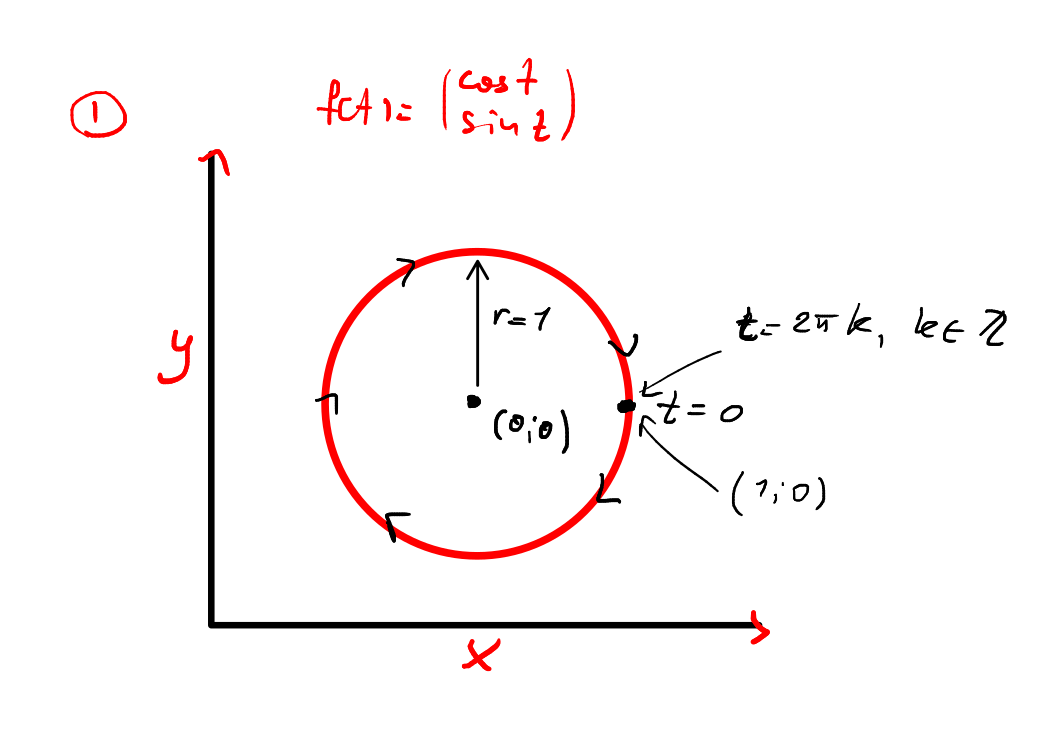
\includegraphics[width=0.8\textwidth]{1.7.1.png}
    \centering
\end{figure}


\subsubsection*{b) Матриця Якобі}
\begin{align*}
    Jf = \begin{pmatrix}
        -\sin t \\ \cos t
    \end{pmatrix}
\end{align*}

\subsubsection*{c) Формули дотичного відображення}
\[Tf : T\R \to T\R^2\]
\begin{align*}
    (Tf)(t, v) = \left((\cos t, \sin t), (-\sin(t) \cdot v , \cos(t) \cdot v)\right)
\end{align*}

\subsubsection*{d) Ранг дотичного відображення в точці}
\[T_{t}f: T_{t}\R \to T_{f(t)}\R^2\]
\[T_{t}f(v) = (-\sin(t) \cdot v , \cos(t) \cdot v)\]

Ранг 0.
\[-\sin(t) = \cos(t) = 0\]
Відомо, що $\sin(t)$ та $\cos(t)$ не мають спільних коренів. \\
Таким чином \colorbox{yellow}{дотичне відображення не має ранг 0 в жодній точці}

Ранг 1.\\
Вся решта точок, тобто \colorbox{yellow}{відображення має ранг 1 $\forall t \in \R$}


\subsection*{Ex 1.7.2}
\[f(t) = (t, t^2)\]

\subsubsection*{a) схематично зобразити криву на площині}
\begin{figure}[h]
    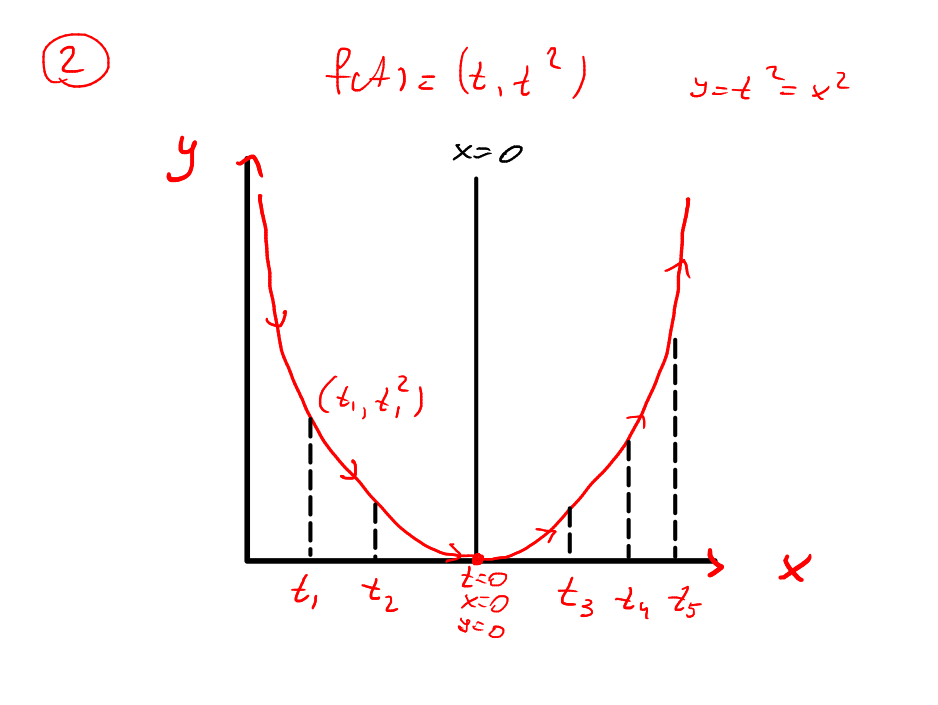
\includegraphics[width=0.8\textwidth]{1.7.2.png}
    \centering
\end{figure}


\subsubsection*{b) Матриця Якобі}
\begin{align*}
    Jf = \begin{pmatrix}
        1 \\ 2t
    \end{pmatrix}
\end{align*}

\subsubsection*{c) Формули дотичного відображення}
\[Tf : T\R \to T\R^2\]
\begin{align*}
    (Tf)(t, v) = \left((t, t^2), (v , 2tv)\right)
\end{align*}

\subsubsection*{d) Ранг дотичного відображення в точці}
\[T_{t}f: T_{t}\R \to T_{f(t)}\R^2\]
\[T_{t}f(v) = (v , 2tv)\]

Ранг 0.
\[1 = 2t = 0\]
Одиниця є констатною.
Таким чином \colorbox{yellow}{дотичне відображення не має ранг 0 в жодній точці}

Ранг 1.\\
Вся решта точок, тобто \colorbox{yellow}{відображення має ранг 1 $\forall t \in \R$}


\subsection*{Ex 1.7.3}
\[f(t) = (t^2, t^3)\]

\subsubsection*{a) схематично зобразити криву на площині}
\begin{figure}[h]
    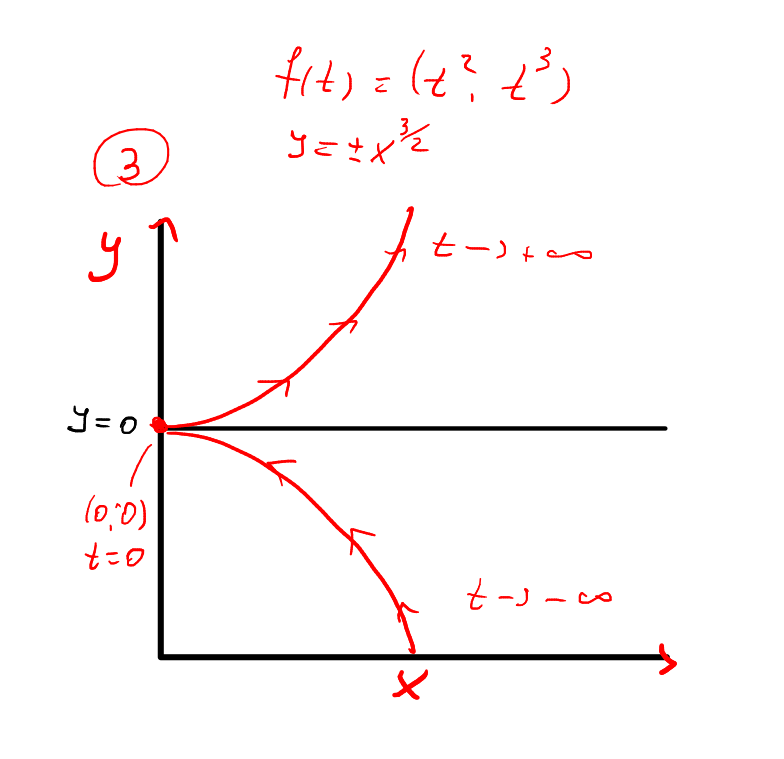
\includegraphics[width=0.8\textwidth]{1.7.3.png}
    \centering
\end{figure}


\subsubsection*{b) Матриця Якобі}
\begin{align*}
    Jf = \begin{pmatrix}
        2t \\ 3t^2
    \end{pmatrix}
\end{align*}

\subsubsection*{c) Формули дотичного відображення}
\[Tf : T\R \to T\R^2\]
\begin{align*}
    (Tf)(t, v) = \left((t^2, t^3), (2tv, 3t^2v)\right)
\end{align*}

\subsubsection*{d) Ранг дотичного відображення в точці}
\[T_{t}f: T_{t}\R \to T_{f(t)}\R^2\]
\[T_{t}f(v) = (2tv, 3t^2v)\]

Ранг 0.
\[2t = 3t^2 = 0\]
\[t = 0\]
Таким чином \colorbox{yellow}{дотичне відображення має ранг 0 лише в точці $t=0$}

Ранг 1.\\
Вся решта точок, тобто \colorbox{yellow}{відображення має ранг 1 $\forall t \in \R, t\ne 0$}



\subsection*{Ex 1.7.4}
\[f(t) = (\sin(t), t^2)\]

\subsubsection*{a) схематично зобразити криву на площині}
\begin{figure}[h]
    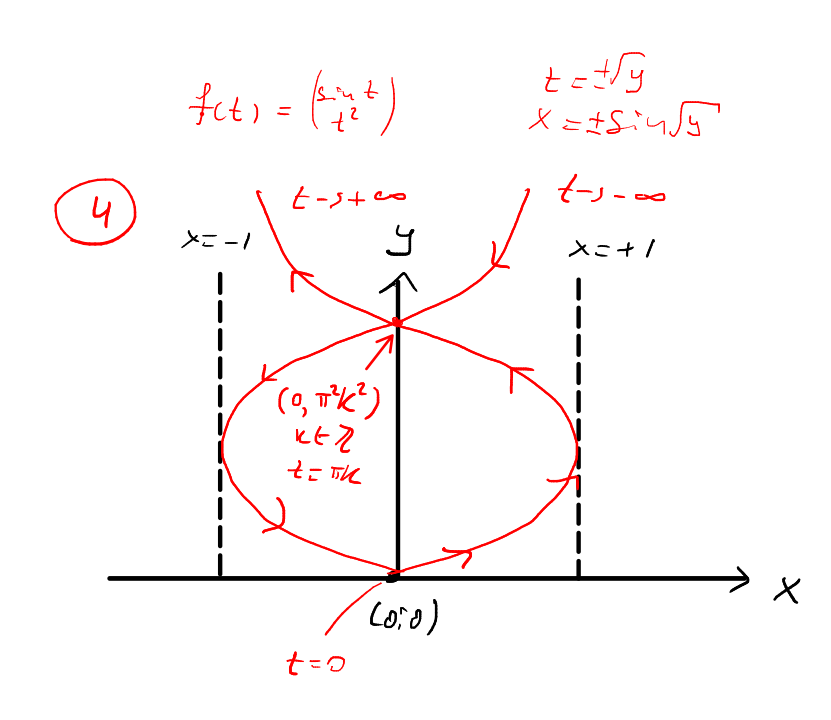
\includegraphics[width=0.8\textwidth]{1.7.4.png}
    \centering
\end{figure}


\subsubsection*{b) Матриця Якобі}
\begin{align*}
    Jf = \begin{pmatrix}
        \cos(t) \\ 2t
    \end{pmatrix}
\end{align*}

\subsubsection*{c) Формули дотичного відображення}
\[Tf : T\R \to T\R^2\]
\begin{align*}
    (Tf)(t, v) = \left((\sin(t), t^2), (\cos(t)v, 2tv)\right)
\end{align*}

\subsubsection*{d) Ранг дотичного відображення в точці}
\[T_{t}f: T_{t}\R \to T_{f(t)}\R^2\]
\[T_{t}f(v) = (\cos(t)v, 2tv)\]

Ранг 0.
\[\cos(t) = 2t = 0\]
\[t = 0\]
Таким чином \colorbox{yellow}{дотичне відображення має ранг 0 лише в точці $t=0$}

Ранг 1.\\
Вся решта точок, тобто \colorbox{yellow}{відображення має ранг 1 $\forall t \in \R, t\ne 0$}



\end{document}

